\chapter{Methodology}\label{chapter:methodology}
A high-level overview of the study performed on the relative effect of the \glspl{vdp} of \glspl{hcv} is as follows:

\begin{enumerate}\addtolength{\itemsep}{0.5\baselineskip}
\item Develop a set of baseline combinations to represent a range of highly productive \glspl{hcv}.
\item Define reasonable ranges for each pertinent \gls{vdp} to be varied within.
\item Evaluate the relative effect of altering each \gls{vdp} within its selected range on overall vehicle performance within the \gls{pbs} framework.
\end{enumerate}

%==============================================
%      SECTION
%==============================================
\section{Baseline Combinations\label{section:methodbaselinecombinations}}
Three baseline \gls{hcv} configurations were developed based on South African workhorse vehicles and Australia's most common PBS vehicle.  Previous \gls{pbs} assessments conducted by \gls{wits} and the \gls{csir} were used to develop the design of each of the baseline combinations.

The same high-level prime mover was used for each baseline, with adjustments to the wheelbase where necessary. A set of representative suspensions were developed and used for all combinations to avoid inserting any bias from discrepancies between the baseline suspension designs. Sections \ref{section:baseline-quad-semi} to \ref{section:baseline-rigid-drawbar-combination} detail the development of each baseline vehicle configuration.

%==============================================
%      SECTION
%==============================================
\section{\gls{vdp} ranges\label{section:methodvdpranges}}
To define reasonable upper and lower limits for each pertinent \gls{vdp}, \gls{oem} variations, legal restrictions, physical constraints, global studies, and data from \gls{pbs} assessments previously conducted by Wits were consolidated and consulted. Details on how the range for each pertinent \gls{vdp} was chosen are contained in Section~\ref{chapter:parameter-range-selection}.

The geometrical limits of a \gls{hcv} are largely governed by the prescriptive legislation of the country in which the combination will be operating.The South African legislation was chosen for developing the geometrical limits to provide value to the \gls{pbs} pilot project in South African. This would not limit the results to being applicable only in South Africa, but if used internationally, the local legislation should be consulted to determine where results may differ.

Inertial, suspension and tyre properties are not widely available which is one of the factors that drive the need for this research. \gls{oem} variations, data from PBS assessments conducted by Wits and Global studies were consulted and the information was consolidated to develop ranges for each of the pertinent \glspl{vdp} that would represent the global \gls{hcv} fleet as local legislation does not dictate any restrictions on the origins of \gls{hcv} components.

%==============================================
%      SECTION
%==============================================
\section{Evaluating \gls{vdp} Relative Influence}

To evaluate the relative influence of each \gls{vdp} on each of the baseline combinations, the \glspl{vdp} were varied in isolation while keeping all other \glspl{vdp} constant at their baseline value. To evaluate the influence of each \gls{vdp}, the \gls{vdp} was varied by 5 evenly distributed points from its maximum to minimum value within its range as determined in Section~\ref{chapter:parameter-range-selection}. This resulted in a total of 8345 simulations being run in \trucksim{} as illustrated in Figure~\ref{figure:number-of-simulations-overview}.

%----------------------------------------------
%      FIGURE
%----------------------------------------------
\begin{figure}[H]
	\centering
	\includegraphics[width=1\textwidth]{fig/Number-of-simulations-Infographic}
	\caption{Overview of the number of \gls{hcv} simulations performed}
	\label{figure:number-of-simulations-overview}
\end{figure}
%----------------------------------------------
%      FIGURE
%----------------------------------------------

\trucksim{} was used as the multi-body vehicle dynamics simulation package to simulate the \gls{hcv} performing a set of \gls{pbs} manoeuvres. The simulation results were used to determine the safety of each \gls{hcv} within the \gls{pbs} framework using a post processor developed in \matlab{} at \gls{wits}. A \matlab{} script automated the adjustment of each individual or combination of parameters within a \trucksim{} model according to the work flow illustrated in Figure~\ref{figure:matlab-trucksim-api-interaction} allowing for the simulation of a large set of vehicle configurations. The versions of each software packaged used are included in Section~\ref{section:software}.

The simulation software and models were calibrated using results published by the \gls{ntc} as detailed in Section~\ref{section:validation-method}.

%----------------------------------------------
%      FIGURE
%----------------------------------------------
\begin{figure}[H]
	\centering
	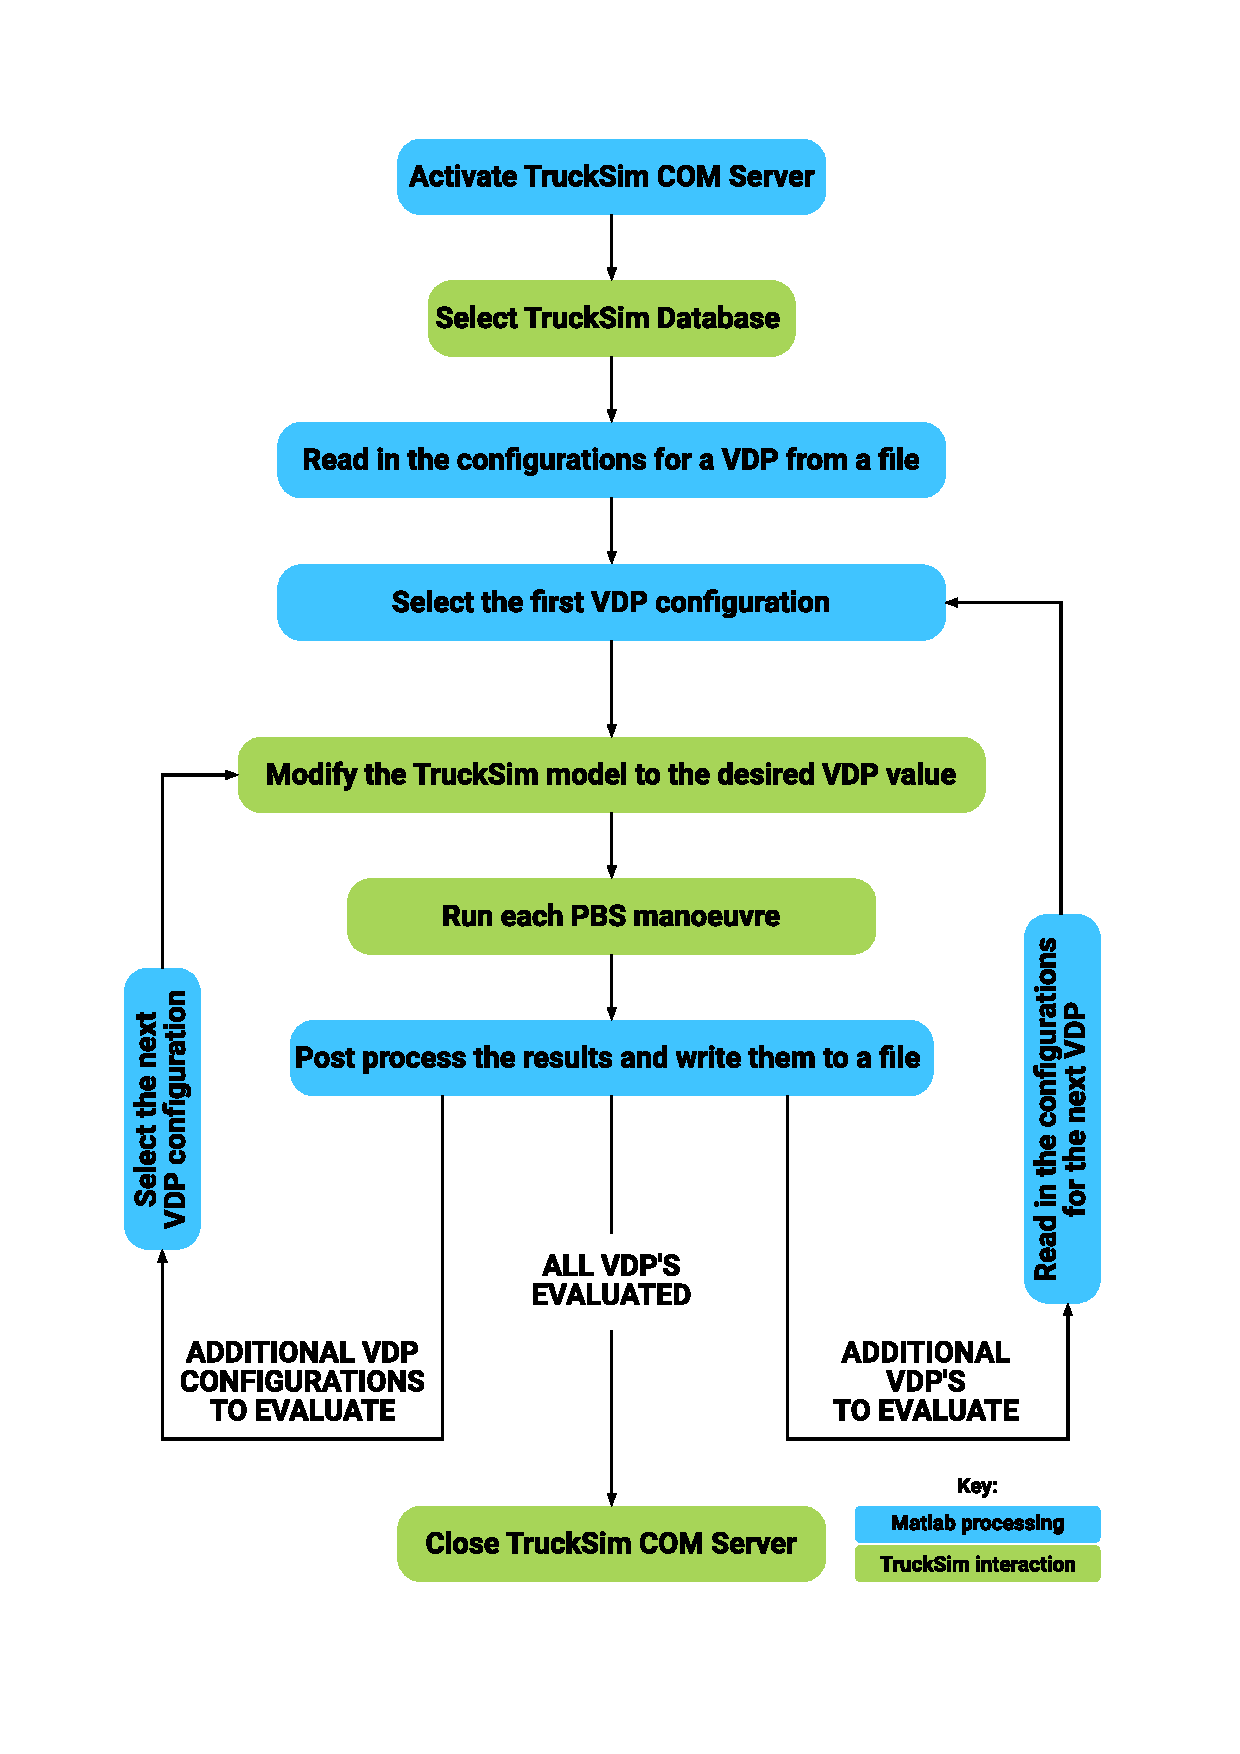
\includegraphics[width=0.75\textwidth]{fig/2018-03-23_trucksim-com-server-flowchart}
	\caption{\matlab{} interaction with the \trucksim{} 2018 API using a COM server}
	\label{figure:matlab-trucksim-api-interaction}
\end{figure}
%----------------------------------------------
%      FIGURE
%----------------------------------------------

%==============================================
%      SECTION
%==============================================
\section{Software}\label{section:software}

The following software packages were used to perform the vehicle simulations:

\begin{enumerate}
	\item \textbf{\trucksim{} 2018 \cite{MechanicalSimulation2016}:} a multi-body vehicle dynamics package used to simulate the various \gls{hcv} vehicle configurations performing the \gls{pbs} manoeuvres.
	\item \textbf{\matlab{} 2018 \cite{MATHWORKS2015}:} a high-level coding environment capable of performing numerical computation and visualisation. Matlab was used in two ways; to post process the simulation outputs of the \trucksim{} simulations and determine vehicle performance within the \gls{pbs} framework and to compare the relative effect of each \gls{vdp} on vehicle performance.
\end{enumerate}

%==============================================
%      SECTION
%==============================================
\section{Software Calibration}\label{section:validation-method}

To perform real world testing to validate the software used to evaluate the \gls{pbs} performance of \glspl{hcv}, experts in the industry were consulted to determine the costs that would be involved. 

In the cost analysis, KDG logistics was consulted to get a quotation of the cost to hire a 6 car car-carrier with a driver and Gerotek was contacted to get a quotation for the use of their test track and tilt-table facilities. An estimated minimum time required to perform the physical testing is included in Table~\ref{table:est-min-time-physical-pbs-testing} (taking into account safety precautions, fitting and testing of sensors that would be used to acquire the data required for validation) and the projected costs of physical testing of a single \gls{hcv} is summarised in Table~\ref{table:est-cost-physical-pbs-testing}. 

The author would like to thank KDG Logistics and Gerotek for their time and efforts involved in providing the quotations.

%----------------------------------------------
%      TABLE
%----------------------------------------------
\begin{table}[H]
	\centering\footnotesize
	\begin{threeparttable}

		\begin{tabulary}{\textwidth}{cc}
			\toprule
\textbf{Manoeuvre}                     & \textbf{Estimated Time Required to Test} \\
			\midrule
Low-speed turn                         & 4 hours                          \\
High-speed lane-change                 & 4 hours                          \\
High-speed tracking on a straight path & 4 hours                          \\
Pulse-steer test                       & 4 hours                          \\
Tilt-table                             & 8 hours                          \\
			\bottomrule
		\end{tabulary}

		\caption{Estimation of the minimum time required to perform physical PBS testing}
		\label{table:est-min-time-physical-pbs-testing}

		%\begin{tablenotes}
		%\item[1] %\tnote{1}
		%\end{tablenotes}

	\end{threeparttable}
\end{table}
%----------------------------------------------
%      TABLE
%----------------------------------------------

Additional funding of R 145 704.00 was not available for validating the software used with the physical testing of a \gls{hcv}. \trucksim{} indicates that their software has been validated and correclated to extensive real-world results as measured and observed by a multitude of well-known automotive \glspl{oem} such as Izuzu, Ford and Toyota along with many others \cite{MechanicalSimulation2018}. Thus, considering the objective of this study is to determine the relative influence of pertinent \glspl{vdp} used as input parameters in multi-body vehicle dynamics simulation software, it was deemed suitable to omit real-world testing and validation and instead perform a calibration of the software according to a framework provided for \gls{pbs} assessors to ensure their simulations are providing accurate results of vehicle safety performance.

%----------------------------------------------
%      TABLE
%----------------------------------------------
\begin{table}[H]
	\centering\footnotesize
	\begin{threeparttable}

		\begin{tabulary}{\textwidth}{lccc}
			\toprule
\textbf{Item}          & \textbf{Cost}     & \textbf{Duration}   & \textbf{Total Cost}  \\
			\midrule

KDG Truck (incl. driver) & R 24 000 per day  & 3 days\tnote{1}    & R72 000.00  \\
Payload Cars           & R 1 800 per day\tnote{1}   & 3 days     & R5 400.00   \\
Gerotek Straight track & R 3 019 per hour  & 16 hours & R48 304.00  \\
Tilt-table test        & R 20 000 per test & One test   & R20 000.00  \\
                       &                   & Total      & R145 704.00 \\
			\bottomrule
		\end{tabulary}

		\caption{Estimation of the minimum time required to perform physical PBS testing}
		\label{table:est-cost-physical-pbs-testing}

		\begin{tablenotes}
		\item[1] Assuming 8 hours per day
		\item[2] Assuming 6 rental vehicles at R 300 each (excluding special insurances)
		\item[3] Assuming the tilt-table test can be completed in a single day
		\end{tablenotes}

	\end{threeparttable}
\end{table}
%----------------------------------------------
%      TABLE
%----------------------------------------------

The \gls{ntc} framework was developed by requesting consultants to compare three computer-based modelling packages (ADAMS, AUTOSIM and \glspl{umtri} Yaw/Roll) to evaluate (in isolation of each other) the \gls{pbs} performance of a B-double and truck-trailer heavy vehicle combination \cite{Prem2001} (known as an interlink and rigid drawbar combination in South Africa).

The \gls{ntc} prescribed a set of inputs for a representative B-double and truck-trailer combination used by all consultants. The vehicles were simulated to perform identical pulse steer, step steer, standard SAE lane change and a low-speed 90\degree{} turn manoeuvres.

The B-double was found to have excellent agreement between all three of the modelling packages. The truck-trailer combination is an inherently less stable vehicle and produced larger but still acceptable amounts of variation in results between the modelling packages.

The Yaw/Roll simulation results were provided by the \gls{ntc} for service providers to calibrate their computer-modelling software and techniques. This data was used to validate the models.

\subsection{Software Calibration Results}\label{section:validation-results}

The behaviour of the B-double and truck-trailer simulated in \trucksim{} 2018 was found to have good correlation with the behaviour simulated in \glspl{umtri} yaw/roll program. Similarly to the outcome of the \gls{ntc} validation, the truck-trailer combination compared less favourably than the B-double combination due to it being a less stable configuration.

Differences in simulated behaviour are attributed to improvements to the prediction of heavy vehicle performance with the latest solvers, differences in the driver models and additional degrees of freedom in the \trucksim{} modelling package.

A set of graphs comparing the simulated vehicle behaviour in \trucksim{} 2018 and \glspl{umtri} yaw/roll program are included in Appendix~\ref{appendix:NTC-validation}.